\documentclass{article}
\usepackage{CJKutf8}
\usepackage{multirow}
\usepackage{listings}
\usepackage{graphicx}
\usepackage{subfigure}
\usepackage[colorlinks,linkcolor=red]{hyperref}
\begin{CJK}{UTF8}{gbsn}
\usepackage[framed,numbered,autolinebreaks]{mcode}
\begin{document}
\title{通信系统第四次作业}
\author{王亭午, 无210班, 2012011018}
\date{2015年5月30号}
\maketitle
\section{仿真二: OFDM系统}本次实验参考DVB-T的2K传输模式的参数,仿真一个简单的QPSK OFDM传输系统。
\subsection{仿真过程}
一个简单的基于循环前缀的OFDM系统仿真过程如下。
\subsubsection{发射机部分}
1. 基本参数定义。2. 随机二进制数据产生。3. 串并变换。4. QPSK 调制。5. 载波分配,
即确定K个载波与N点IFFT之间的对应关系。6. IFFT。
7. 保护间隔插入,即产生循环前缀,同时进行并串转换。
\subsubsection{信道部分}
1. 信道;2. AWGN 噪声。
\subsubsection{接收机部分}
1. 保护间隔去除;2. FFT;3. 载波数据提取;4. QPSK 解调;5. 并串变换;6. 误码计算。
\subsubsection{说明}
对于DVB-T的2K来说,载波数K为1705,FFT点数为2048,载波可以按照下图进行分配。
其中2048点IFFT的第1点不分配载波,这样IFFT之后的时域信号无直流分量。 \\
QPSK调制和解调采用自编的qpskmod.m和qpskdemod.m两个文件,其使用方法见 qpsk\_demo\_ev.m文件。
QPSK调制与解调也可以采用MATLAB自带的PSK调制函数 。
参考代码qpsk\_demo\_ev.m 给出了AWGN信道下QPSK调制解调过程,
代码中已实现的部分用红色标注。可在此基础上修改,也可自己重写。
\subsection{实验}
\subsubsection{学习调制和解调函数的使用,掌握基本OFDM系统的仿真原理。}
\subsubsection{简易OFDM传输系统}
根据DVB-T 2K 传输模式的参数,搭建一个简易OFDM传输系统,
采用1/8保护间隔,QPSK调制,不考虑基带成形滤波器、编码和导频插入。\\
这部分的代码完成在DVB\_1.m中,具体如下:
\begin{lstlisting}
% ------------------------------------------------------------
% Written by Tingwu Wang, Tsinghua University
% Homework 4 for the Course Communication System
%
% 2015.6.29
% ------------------------------------------------------------
% the initial of parameters
TU = 224e-6; % us, the time of the symbol
kCarriers = 1705;
nCarriers = 2048;
bandWidth = 7.61e6; % Hz as the band width
guardInterval = [1/4 1/8 1/16 1/32];

% Data Generation
nDataset = 10; % the data should be round times of the carrier numbers 1705 for 
               % simplicity
nTraining = 1;
QPSKmode = 2; % 2 for qpsk, 1 for bpsk
data = rand(1, kCarriers * (nDataset + nTraining) * QPSKmode) > 0.5;
                                           
% QPSK Modulation, remember to normalize the data
[ich, qch] = qpskmod(data, 1, kCarriers * (nDataset + nTraining), QPSKmode);
ich = ich ./ sqrt(2);
qch = qch ./ sqrt(2);

% plot the input symbols
inputSymbol = ich + 1j*qch;              % Complex modulated data
%scatterplot(inputSymbol);

% the channel symbol with CP as guardian interval
lCp = round(nCarriers * guardInterval(2));
channelSymbol = zeros(length(inputSymbol) + lCp * (nDataset + nTraining), 1);

% from sequencial to parallel
for iSets = 1: 1: nDataset + nTraining
    tempSets = zeros(nCarriers, 1);
    tempSets(2:854, 1) = inputSymbol(1 + (iSets - 1) * kCarriers: ...
        1 + (iSets - 1) * kCarriers + 854 - 2);
    tempSets(1197:2048, 1) = inputSymbol(1 + (iSets - 1) * kCarriers + 854 ...
        - 2 + 1: iSets * kCarriers);

    % get the channel symbol, and add the cp
    channelSymbol(lCp + 1 + (iSets - 1) * nCarriers: lCp + iSets * nCarriers) ...
        = ifft(tempSets);
    channelSymbol(1: lCp) = channelSymbol(end - lCp + 1, end);
end
figure(1)
plot(real(channelSymbol));
figure(2)
freqPlot = fft(channelSymbol);
plot(real(freqPlot));
\end{lstlisting}
在上面的情况中,考虑了使用一个周期1705个数据作为抗多径的均衡数据。
\subsubsection{波形和频谱}
测试发射信号的时域波形和频谱\\
我们得到的结果如图,可以看到这个是符合我们的预期的。其中因为我们只使用了2048个子载波中的1705个,我们知道中间的频段应该是空的。
注意数字频率和模拟频率需要乘以一个系数,这里就不详细做了。另外因为我们在\(f=0\)这个载波上值为0,所以我们的信号应该是均值为0的。
\begin{figure}[h]
\begin{minipage}[t]{0.5\linewidth}
\centering
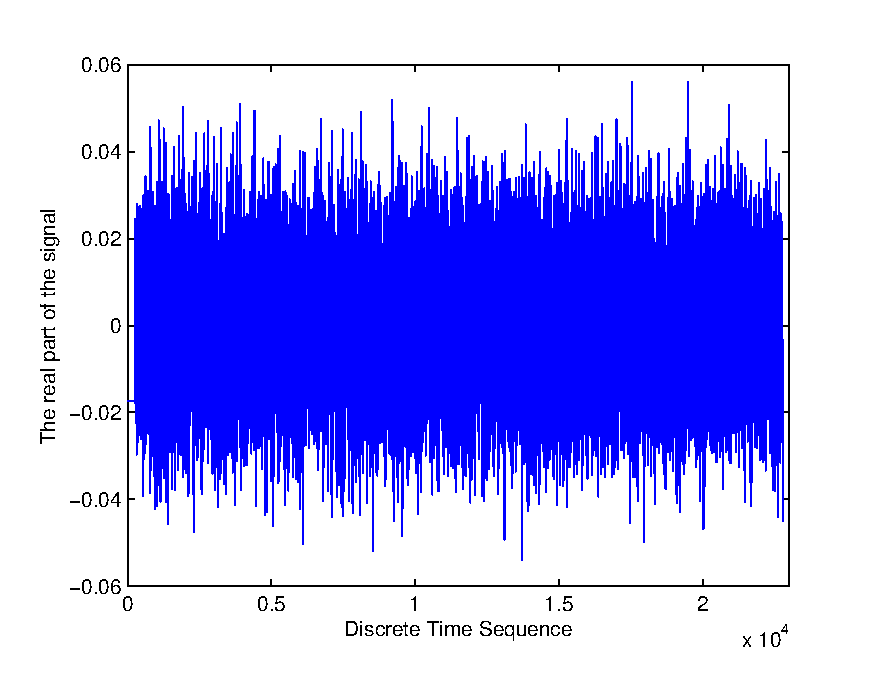
\includegraphics[width=2.2in]{2.eps}
\caption{发射信号的时域波形}
\label{fig:side:a}
\end{minipage}%
\begin{minipage}[t]{0.5\linewidth}
\centering
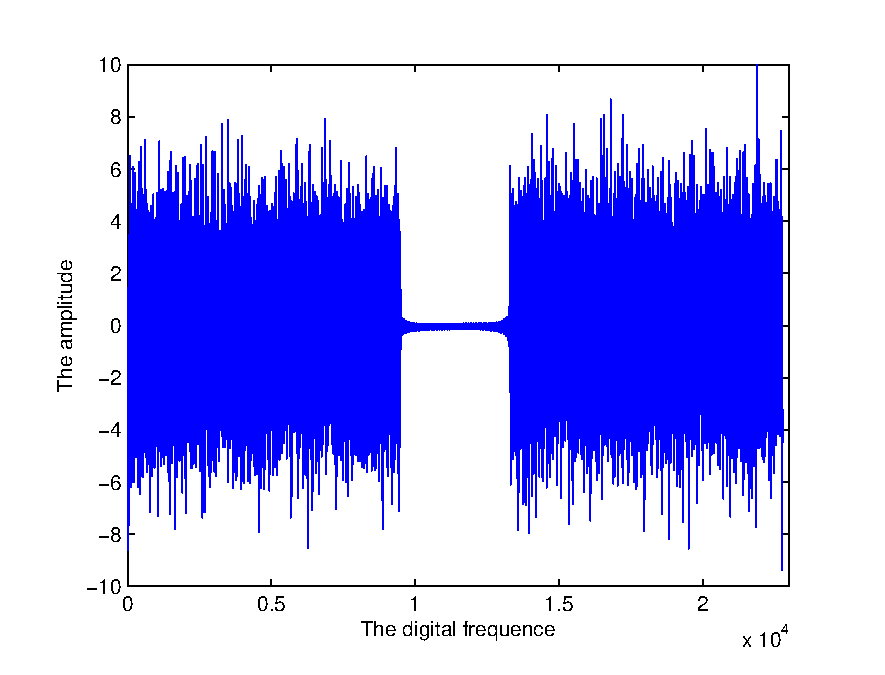
\includegraphics[width=2.2in]{3.eps}
\caption{发射信号的频谱}
\label{fig:side:b}
\end{minipage}
\end{figure}
\subsubsection{AWGN信道}
AWGN信道,在信噪比为8dB的情况下,用scatterplot函数观察、对比进入IF
FT前/后信号的星座图。\\
结果如图,我们获得来进入IFFT之前和之后的图像,分别是Fig. 3和Fig. 4。
可以看到,输入信号是非常规整的QPSK信号,输出IFFT后因为已经变为时域信号,原先的频域特征已经看不出来了。
同时因为噪声的原因,图像变得更加混乱。
\begin{figure}[h]
\begin{minipage}[t]{0.5\linewidth}
\centering
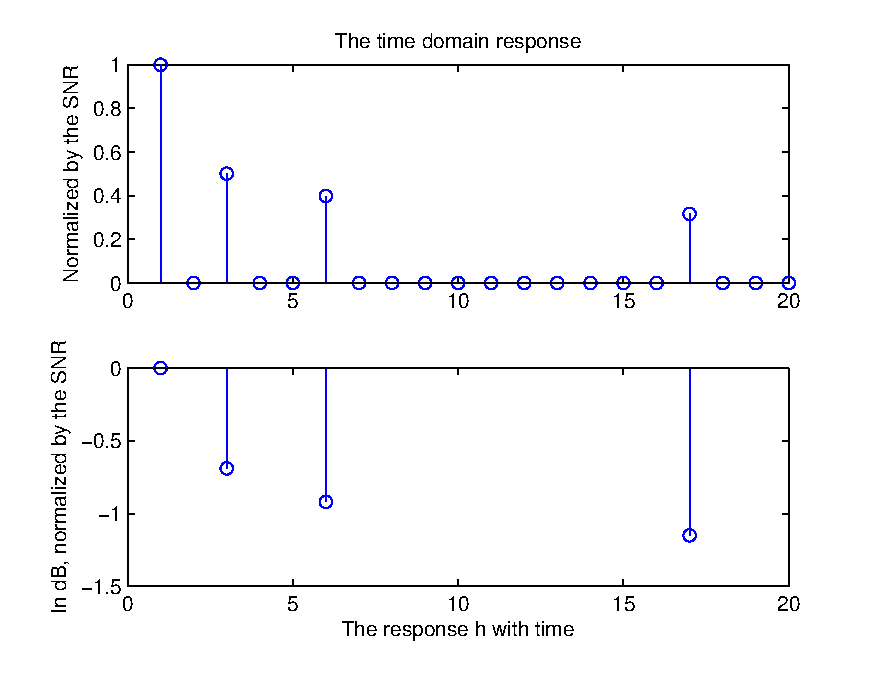
\includegraphics[width=2.2in]{1.eps}
\caption{原始的调制星座图}
\label{fig:side:a}
\end{minipage}%
\begin{minipage}[t]{0.5\linewidth}
\centering
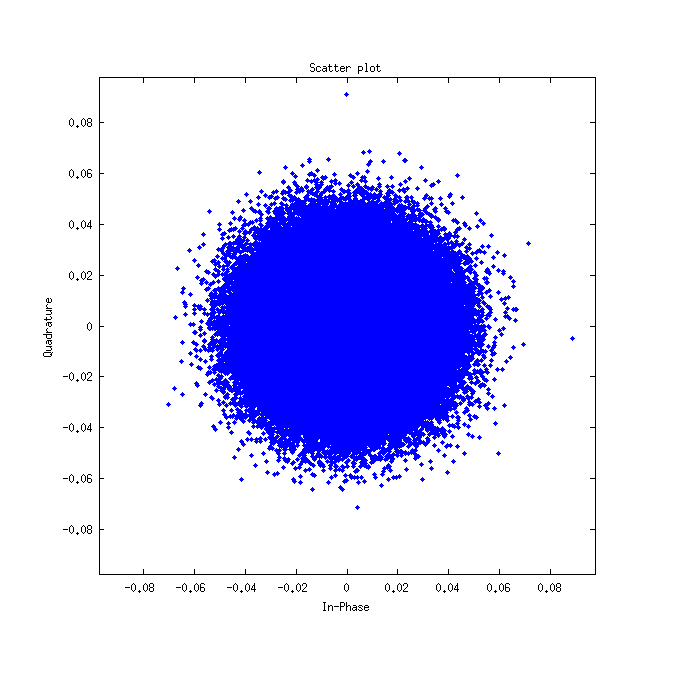
\includegraphics[width=2.2in]{4.eps}
\caption{进入IFFT后叠加了噪声的的调制星座图}
\label{fig:side:b}
\end{minipage}
\end{figure}
\subsubsection{BER-SNR}
AWGN信道。观察不同信噪比下误码率变化情况,画出BER-SNR示意图(误码率\(10^{-1}\)\(10^{-5}\))。
注意误码率较低时需要增加仿真量(至少需要10个误比特)。\\
如Fig. 5图,考虑到这个时候不存在多径效应,因此不需要导频进行均衡。可以看到,随着噪声强度不断增大,误码率越来越高。
\begin{figure}[h]
\centering
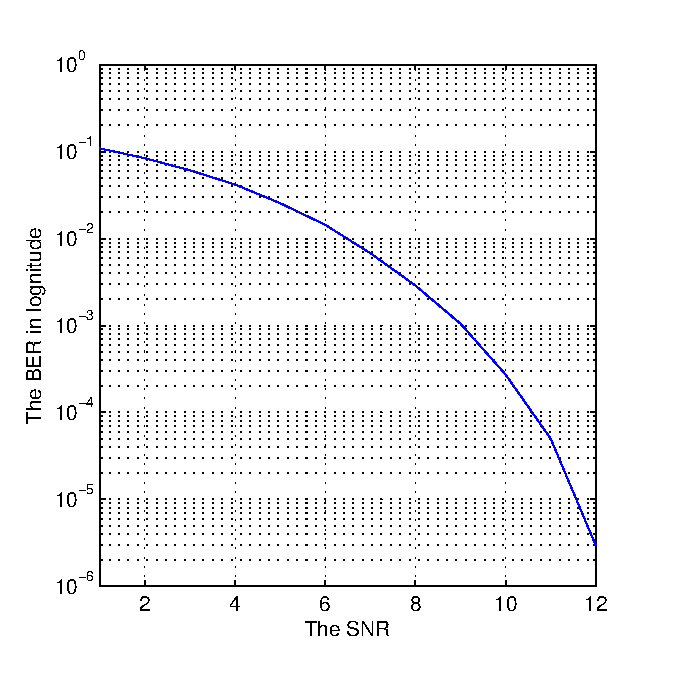
\includegraphics[width=8cm,height = 6cm]{5.eps}
\caption{AWGN信道下的BER曲线}
\end{figure}
\subsubsection{双径信道}
观察不同信噪比下误码率变化情况,画出BER-SNR示意图(误码率\(10^{-1}\)\(10^{-4}\))。
注意误码率较低时需要增加仿真量(至少需要10个误比特)。\\
我们的结果图如下,为Fig. 6。可以看到,我们验证了OFDM在多径的情况下具有抗多径的能力。
为了做演示,我们使用了1705个子载波作为训练数据来计算对应的多径系数。依次根据对角阵的性质计算对应的系数。
然后在后面的数据中使用这个系数来计算消除多径后的结果。
\begin{figure}[t]
\centering
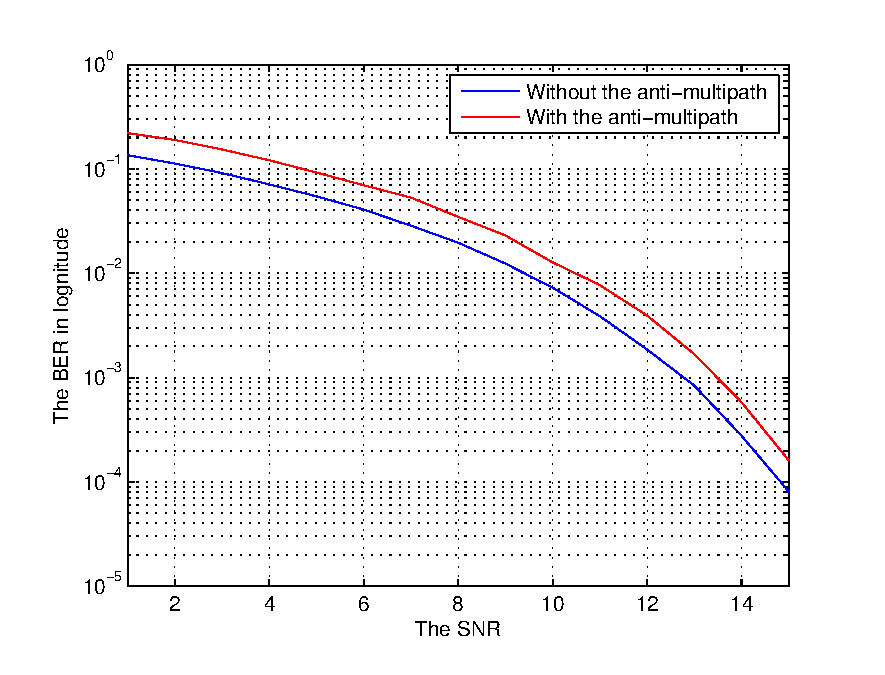
\includegraphics[width=9cm]{6.eps}
\caption{双径信道下的BER曲线}
\end{figure}
\subsubsection{多径信道}
观察不同信噪比下误码率变化情况,画出BER-SNR示意图(误码率\(10^{-1}\)\(10^{-4}\))。
注意误码率较低时需要增加仿真量(至少需要10个误比特)。\\
我们知道,我们现在面对的多径信道实际上是一个最强信号反而不是0延时的那个信号的情况。
因此我们可以遇见,如果直接解码,会存在毁灭性的误差。因此和上面一样,我们进行抗多径的系数计算。
得到的的结果图如下,为Fig. 7。可以看到,我们验证了OFDM在多径的情况下具有抗多径的能力。
如果不做抗多径,直接译码,因为误差来源不是噪声而是延时多径造成的ISI,所以随着噪声减少,译码的结果并不会变好。
\begin{figure}[t]
\centering
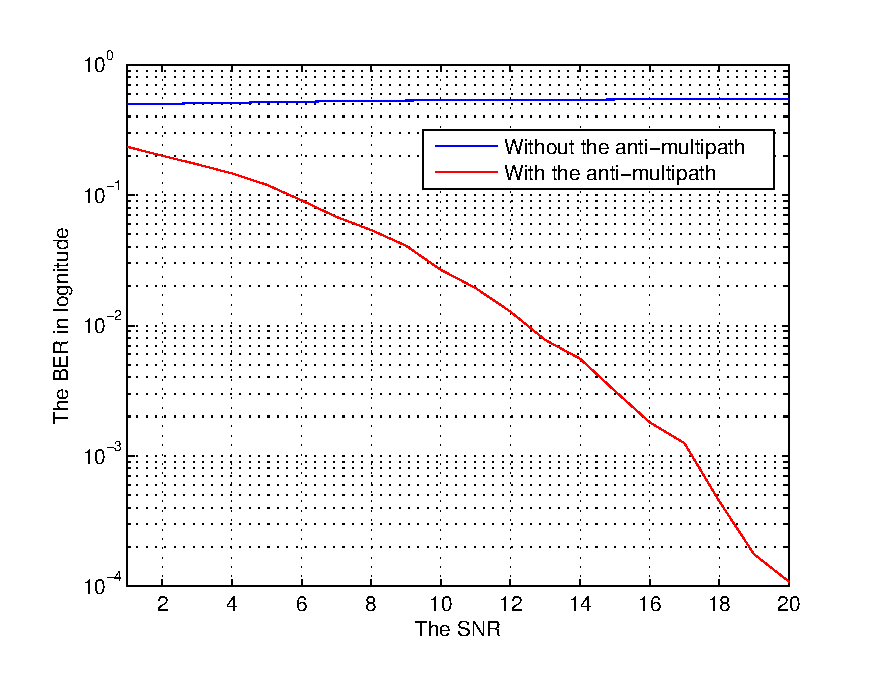
\includegraphics[width=9cm]{7.eps}
\caption{多径信道下的BER曲线}
\end{figure}
\newpage
\section{问答题}
\subsection{时域训练序列、频域分散导频和频域连续导频在信道估计上各有什么优势和局限?}
答案:时域训练序列往往使用数字信号处理的方法,不仅是下面两种方法只在OFDM比较有效,别的方式也可以。但是准确度有一定的劣势。
频域连续导频序列可以在一个时间段上比较密集的训练多径对应的系数,可以很好的应对各种长度的时延扩展,适合比较时不变的信道。
频域分散导频序列相比起来,会消耗更加多的子载波来进行训练,但是可以更加好的应对信道的快速变换。
\subsection{DVB-S2、DVB-T2 相比与 DVB-S 和 DVB-T 有什么新的应用需求,相应做出了什么技术改进?请简述。}
答案:DVB-S2需要在给定带宽内提高数据吞吐率,占用更加少的卫星资源和提高传输能力,更加鲁棒。于是它使用了LDPC方案,和新的调制方案和扩展星座图。\\
DVB-T2需要实现更加灵活多样的业务和动态分配资源。同时需要更加好的单频网性能,能够向后兼容现有的天线系统,更加灵活的带宽和频率规划等等。为了完成这些,它使用了LDPC和不同的OFDM配置,增大OFDM的符号周期,同时使用了256QAM映射,分散导频和T2帧结构,星座旋转等等。
\subsection{数字电视广播中为何出现单频网,其主要技术难点是什么?}
答案:因为现有的频谱是有限的,能利用的则更加的少,新的模式必须要适应已有的PAL信号。为了利用禁用频道,需要使用单频网。
主要难点在于对抗多径,实现在各个发射机的信号频率和时间同步。
\subsection{简述多模光纤与单模光纤在进行传输时的差别。}
答案:多模光纤允许多束光线穿过光纤。因为不同光线进入光纤的角度不同,所以到达光纤末端的时间也不同,产生模色散。
色散限制了多模光纤所能实现的带宽和传输距离,因此多模光纤一般被用于同一办公楼或距离相对较近的区域内的网络连接。
一般采用价格较低的LED作为光源,耦合部件尺寸与多模光纤配合好。\\
单模光纤只允许一束光线穿过光纤。因为只有一种模态,所以不会发生色散。使用单模光纤传递数据的质量更高,传输距离更长。
但是它与光器件的耦合相对困难。一般采用LD或光谱线较窄的LED作为光源,耦合部件尺寸与单模光纤配合好。
\subsection{计算 OFDM 参数}
一个CP-OFDM系统,子载波数为1024,其中导频载波128个,CP长度为64个采样符号(单倍采样)。
CP和数据块组成一帧,一帧时长 0.272ms。采用QPSK调制,2/3码率的LDPC编码。
求系统带宽、频谱利用率和数据传输速率。\\
答案:首先我们有带宽为
\begin{equation}
W = nf = n \frac{1}{T_u} = \frac{1024}{0.272 \times 1024 / (1024 + 64) } = 4\mbox{MHz}
\end{equation}
\begin{equation}
\eta = \frac{1024 - 128}{1024} = 87.5\%
\end{equation}\begin{equation}
\upsilon = 2 \frac{2}{3}\times(1024 - 128) / 0.272 = 4.39\mbox{Mbits/s}
\end{equation}
\end{CJK}
\end{document}